\cohead{\Large\textbf{Schiefe Asymptoten}}
\fakesubsection{Schiefe Asymptoten}
Funktionen vom Typ \(f(x)=\textcolor{blue}{a\cdot e^{kx}}+\textcolor{red}{mx+b}\quad \textcolor{blue}{a},\textcolor{blue}{k}, \textcolor{red}{m}\neq 0\) haben eine schiefe Asymptote. Der erste Teil der Funktion \(\textcolor{blue}{a\cdot e^{kx}}\) geht entweder für sehr große x oder sehr kleine x gegen Null. In diese Richtung nähert sich das Schaubild von \(f(x)\) der Geraden \(\textcolor{red}{mx+b}\) beliebig nahe, d.h. \(\textcolor{red}{y=mx+b}\) ist eine Asymptote von \(f(x)\). Da das Schaubild der Asymptoten nicht mehr parallel zur x-Achse verläuft, spricht man von einer schiefen Asymptoten.

Beispiel: \(f(x)=\textcolor{blue}{2\cdot e^{x}}\textcolor{red}{-x-3}\)

\begin{minipage}{\linewidth}
	\centering
	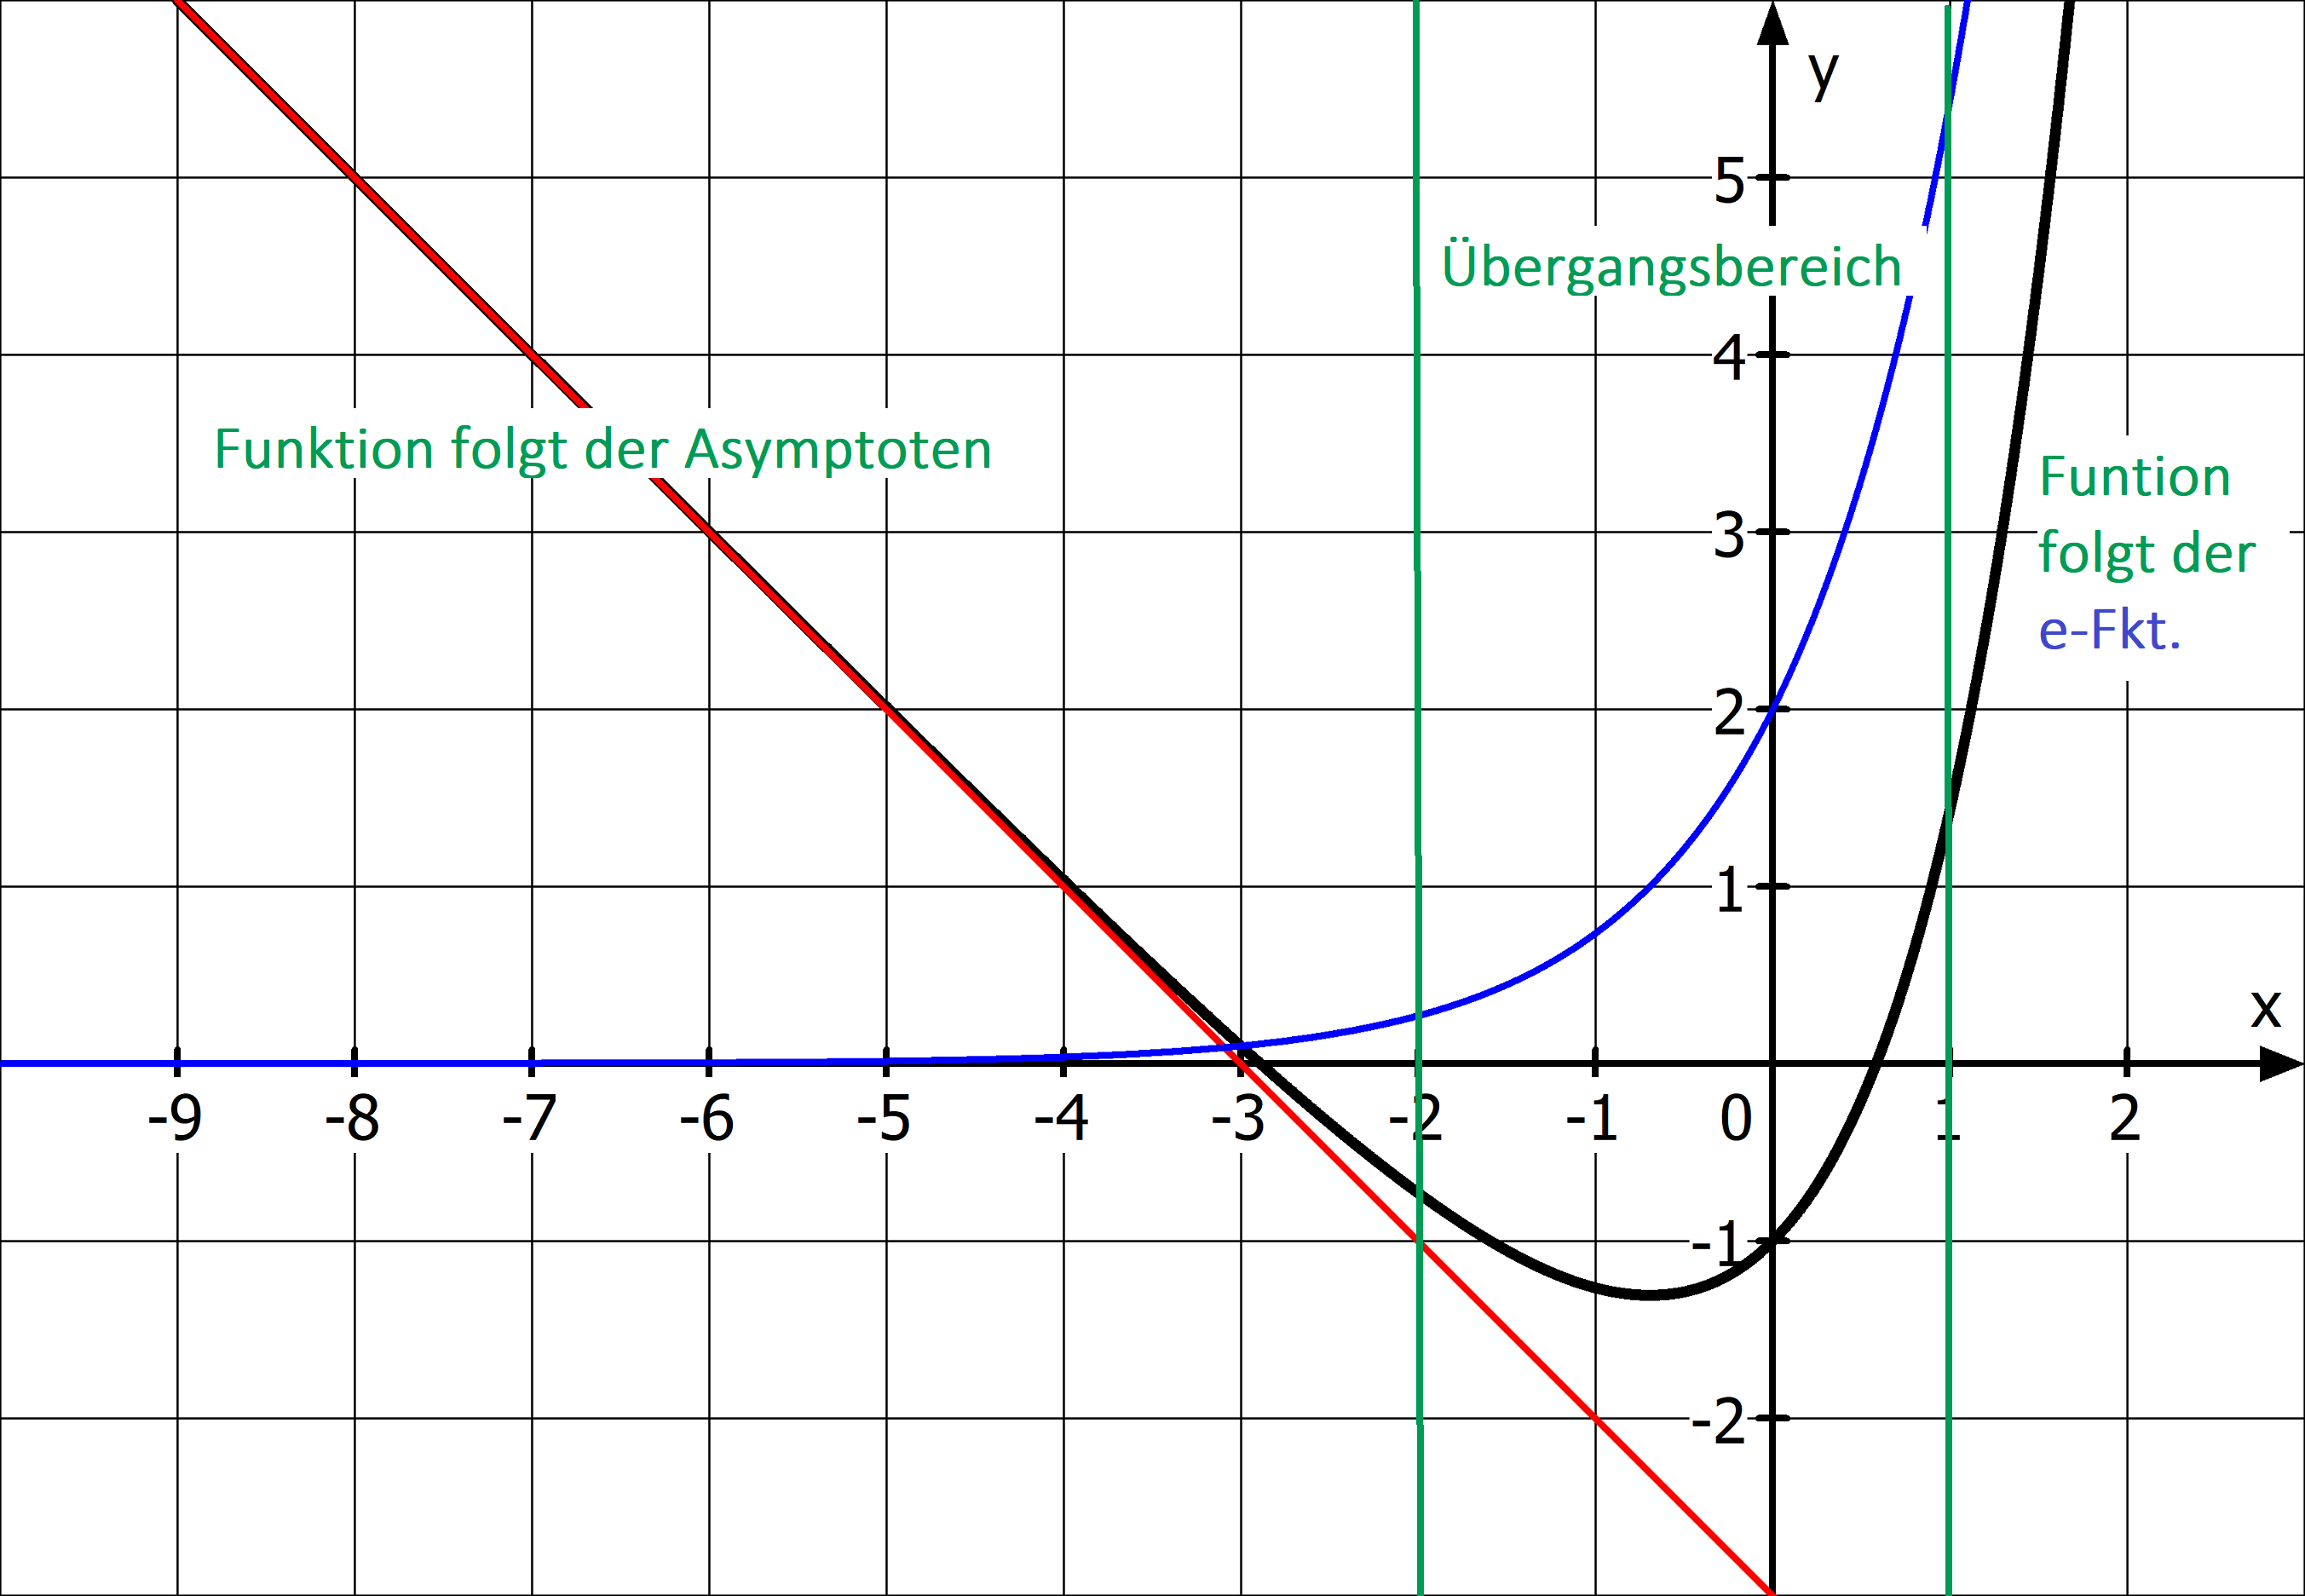
\includegraphics[width=\textwidth]{\eFkt/pics/schiefeAsymptote.png}
\end{minipage}

\smallskip

Die Schaubilder von Funktionen vom obigen Typ lassen sich in 3 Bereiche aufteilen:
\begin{itemize}
	\item In dem Bereich, in dem \textcolor{blue}{\(a\cdot e^{kx}\)} gegen Null geht, folgt die Funktion der \textcolor{red}{Asymptoten}. Im Beispiel ist dies für ca. \(x<-2\) der Fall.
	\item In dem Bereich, in dem \textcolor{blue}{\(a\cdot e^{kx}\)} gegen \(+\infty\) oder \(-\infty\) geht, folgt die Funktion \textcolor{blue}{\(a\cdot e^{kx}\)} Im Beispiel ist dies ab ca. \(x>1\) der Fall.
	\item Im Übergangsbereich zwischen den beiden Bereichen muss man die beiden Teile mit einem Bogen miteinander verbinden.
\end{itemize}
Das obige Beispiel hat einen Tiefpunkt bei ca. \(x\approx -0,8\). Mit Hilfe der Ableitung werden wir in Zukunft Hoch- und Tiefpunkte berechnen können. Die obige Funktion hat 2 Nullstellen, die man jedoch nicht exakt bestimmen kann.
\begin{tcolorbox}
	Gleichungen vom Typ

	$\makebox[\linewidth]{\(ae^{kx}+mx+b=0\)}$
	sind im Allgemeinen nicht exakt lösbar. Man kann lediglich die Lösungen auf beliebig viele Nachkommastellen bestimmen.
\end{tcolorbox}
\newpage
%%%%%%%%%%%%%%%%%%%%%%%%%%%%%%%%%%%%%%%%%%%%%%%%%%%%%%%%%%%%%%%%%%%%%%%%%%%%%%%%%%%%%%%%%%%%%%%%%%%%%%
\begin{Exercise}[title={Skizziere die Asymptote, den Teil mit \(ae^{kx}\) sowie das Schaubild der Funktion.}, label=schAsyA1]

    \begin{minipage}{\textwidth}
		\begin{enumerate}[label=\alph*)]
			\item \(f_1(x)=e^{-x}+2x-3\)
			\item \(f_2(x)=-e^{-2x}+0,5x\)
			\item \(f_3(x)=-e^{x}-\frac{2}{3}x+1\)
			\item \(f_4(x)=-2e^{-x}-2x+1\)
			\item \(f_5(x)=3e^{1,4x}+\frac{3}{4}x-1\)
			\item \(f_6(x)=e^{2x}+0,4x-3\)
			\item \(f_7(x)=-3e^{-0,5x}-x\)
			\item \(f_8(x)=-2e^{4x}+\frac{4}{3}x+5\)
		\end{enumerate}
    \end{minipage}
\end{Exercise}
%%%%%%%%%%%%%%%%%%%%%%%%%%%%%%%%%%%%%%%%%
\begin{Answer}[ref=schAsyA1]

	\begin{minipage}{\textwidth}
		\begin{minipage}{0.5\textwidth}
			\begin{enumerate}[label=\alph*)]
				\item \(f_1(x)=e^{-x}+2x-3\)

                \begin{minipage}[t]{0.87\textwidth}
					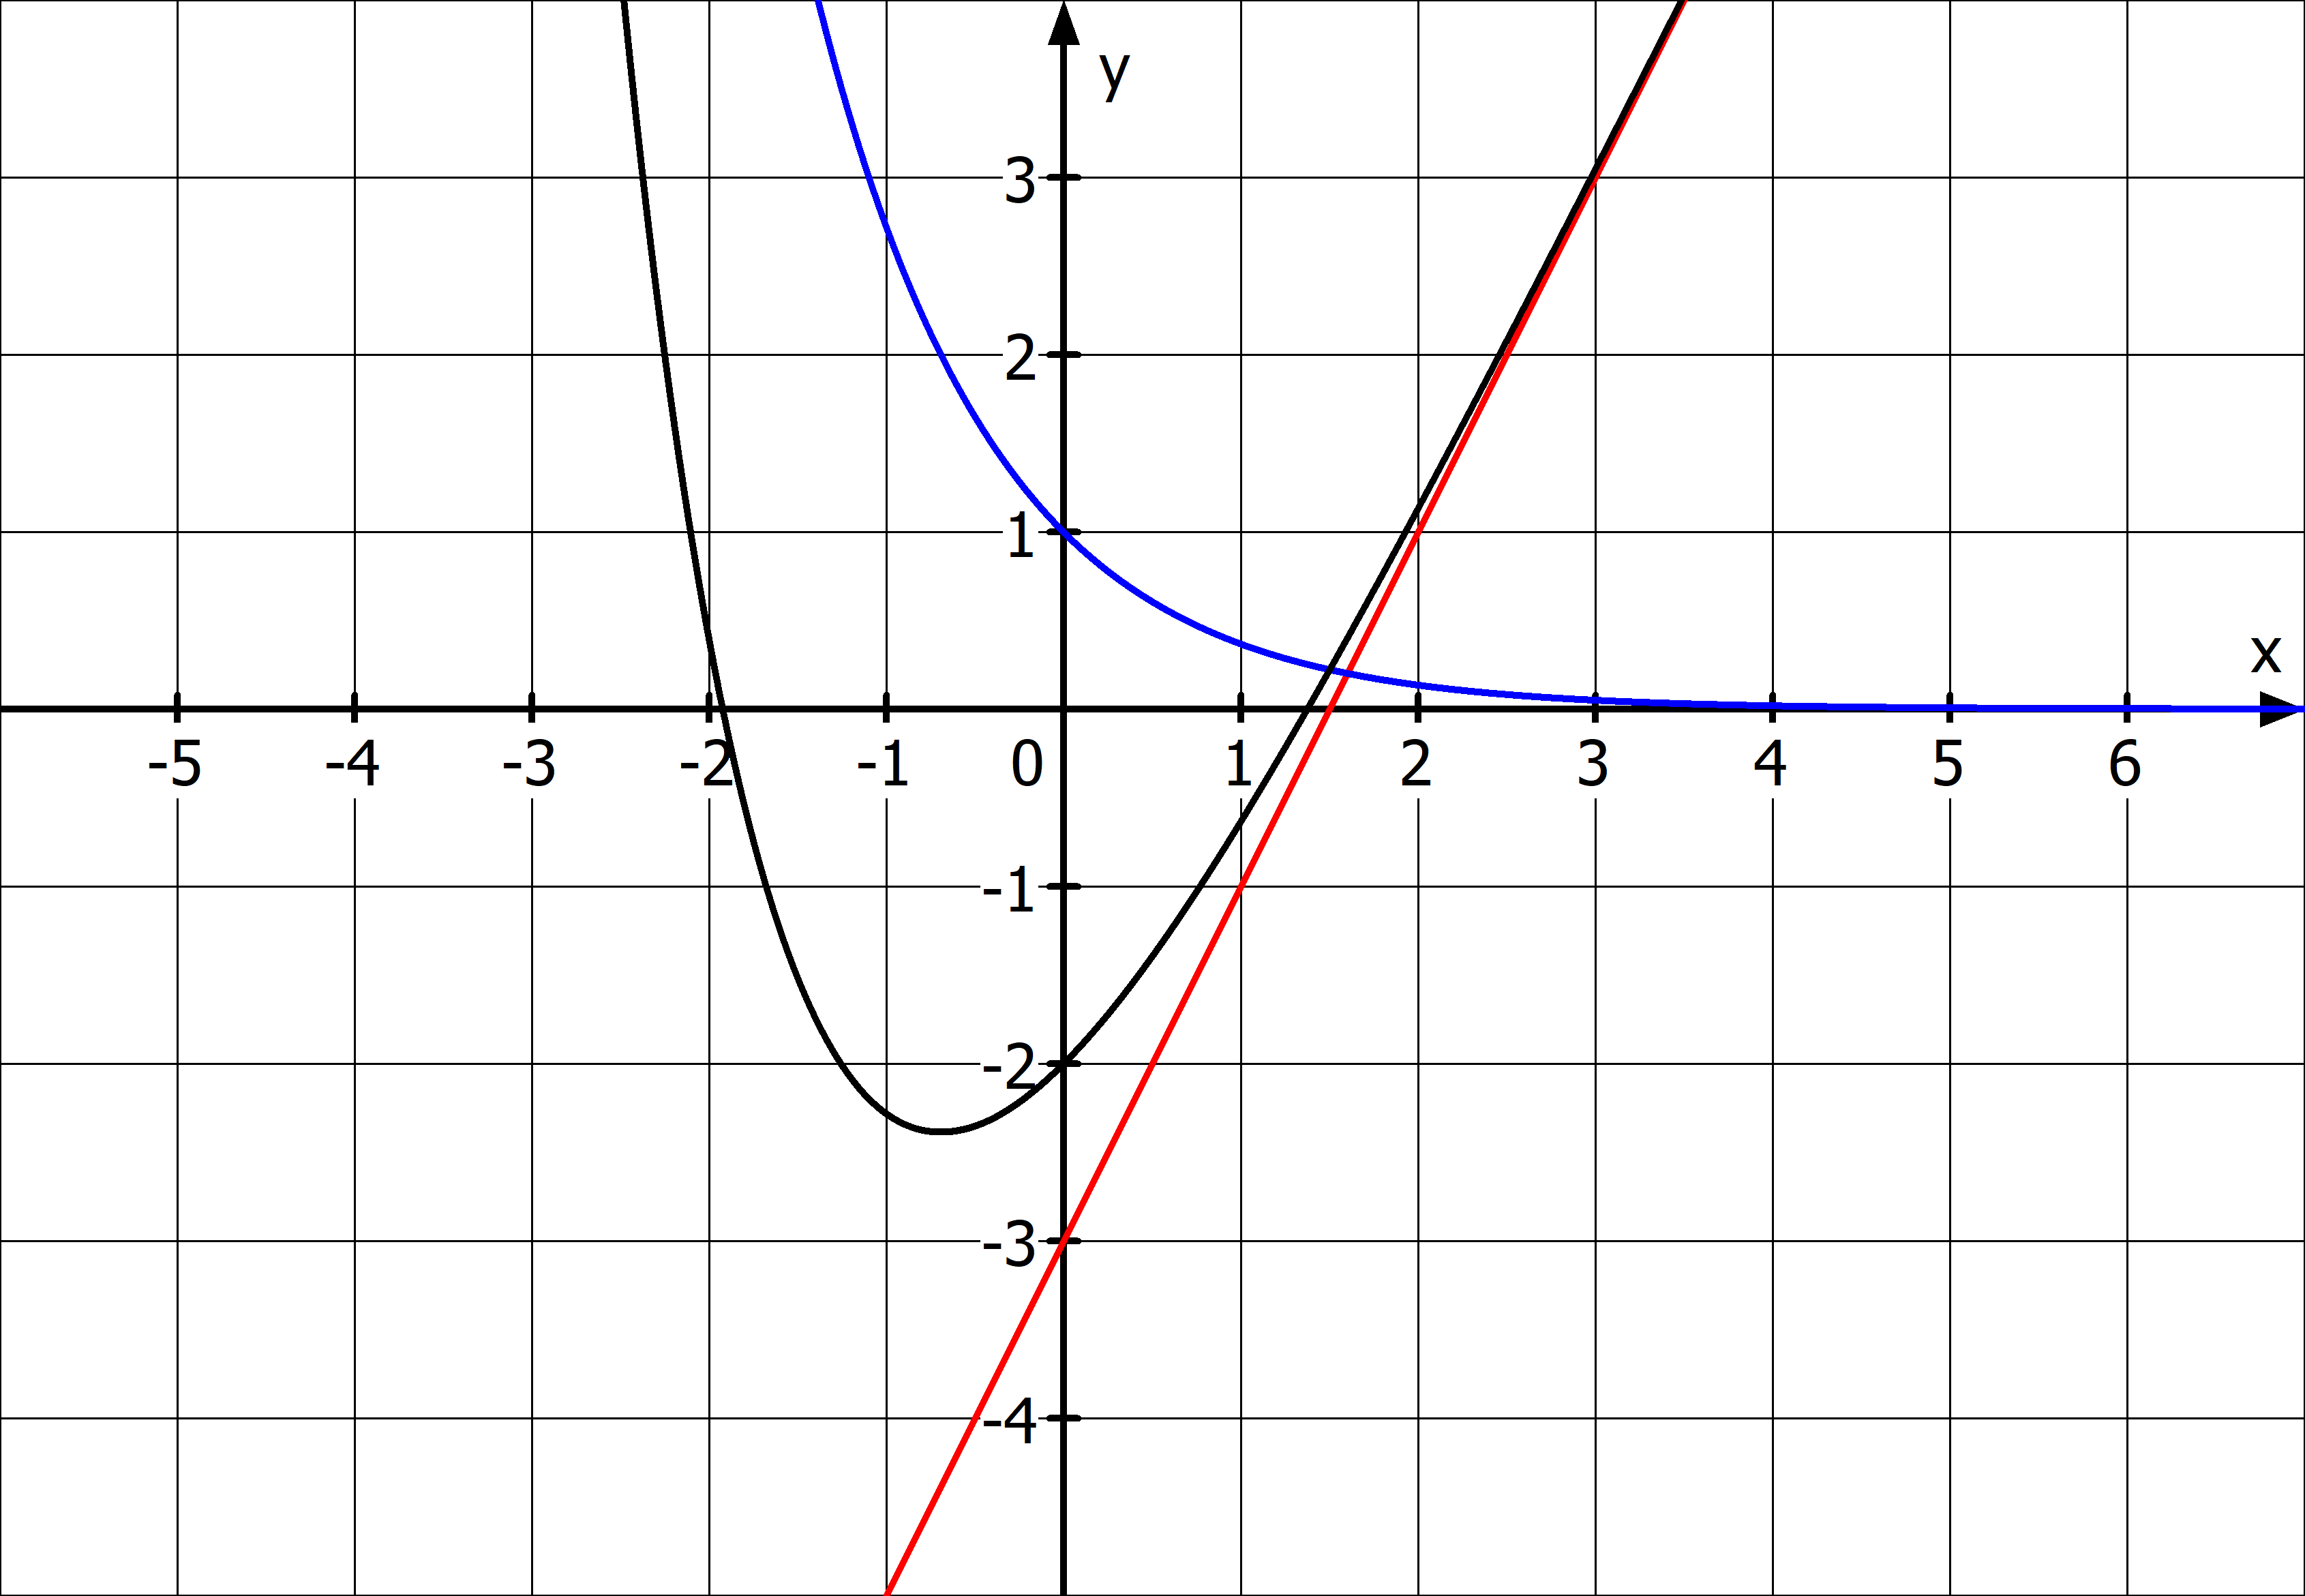
\includegraphics[width=\linewidth]{\eFkt/pics/schiefeAsymptoteA1.png}
				\end{minipage}
				\item \(f_2(x)=-e^{-2x}+0,5x\)

                \begin{minipage}[t]{0.87\textwidth}
					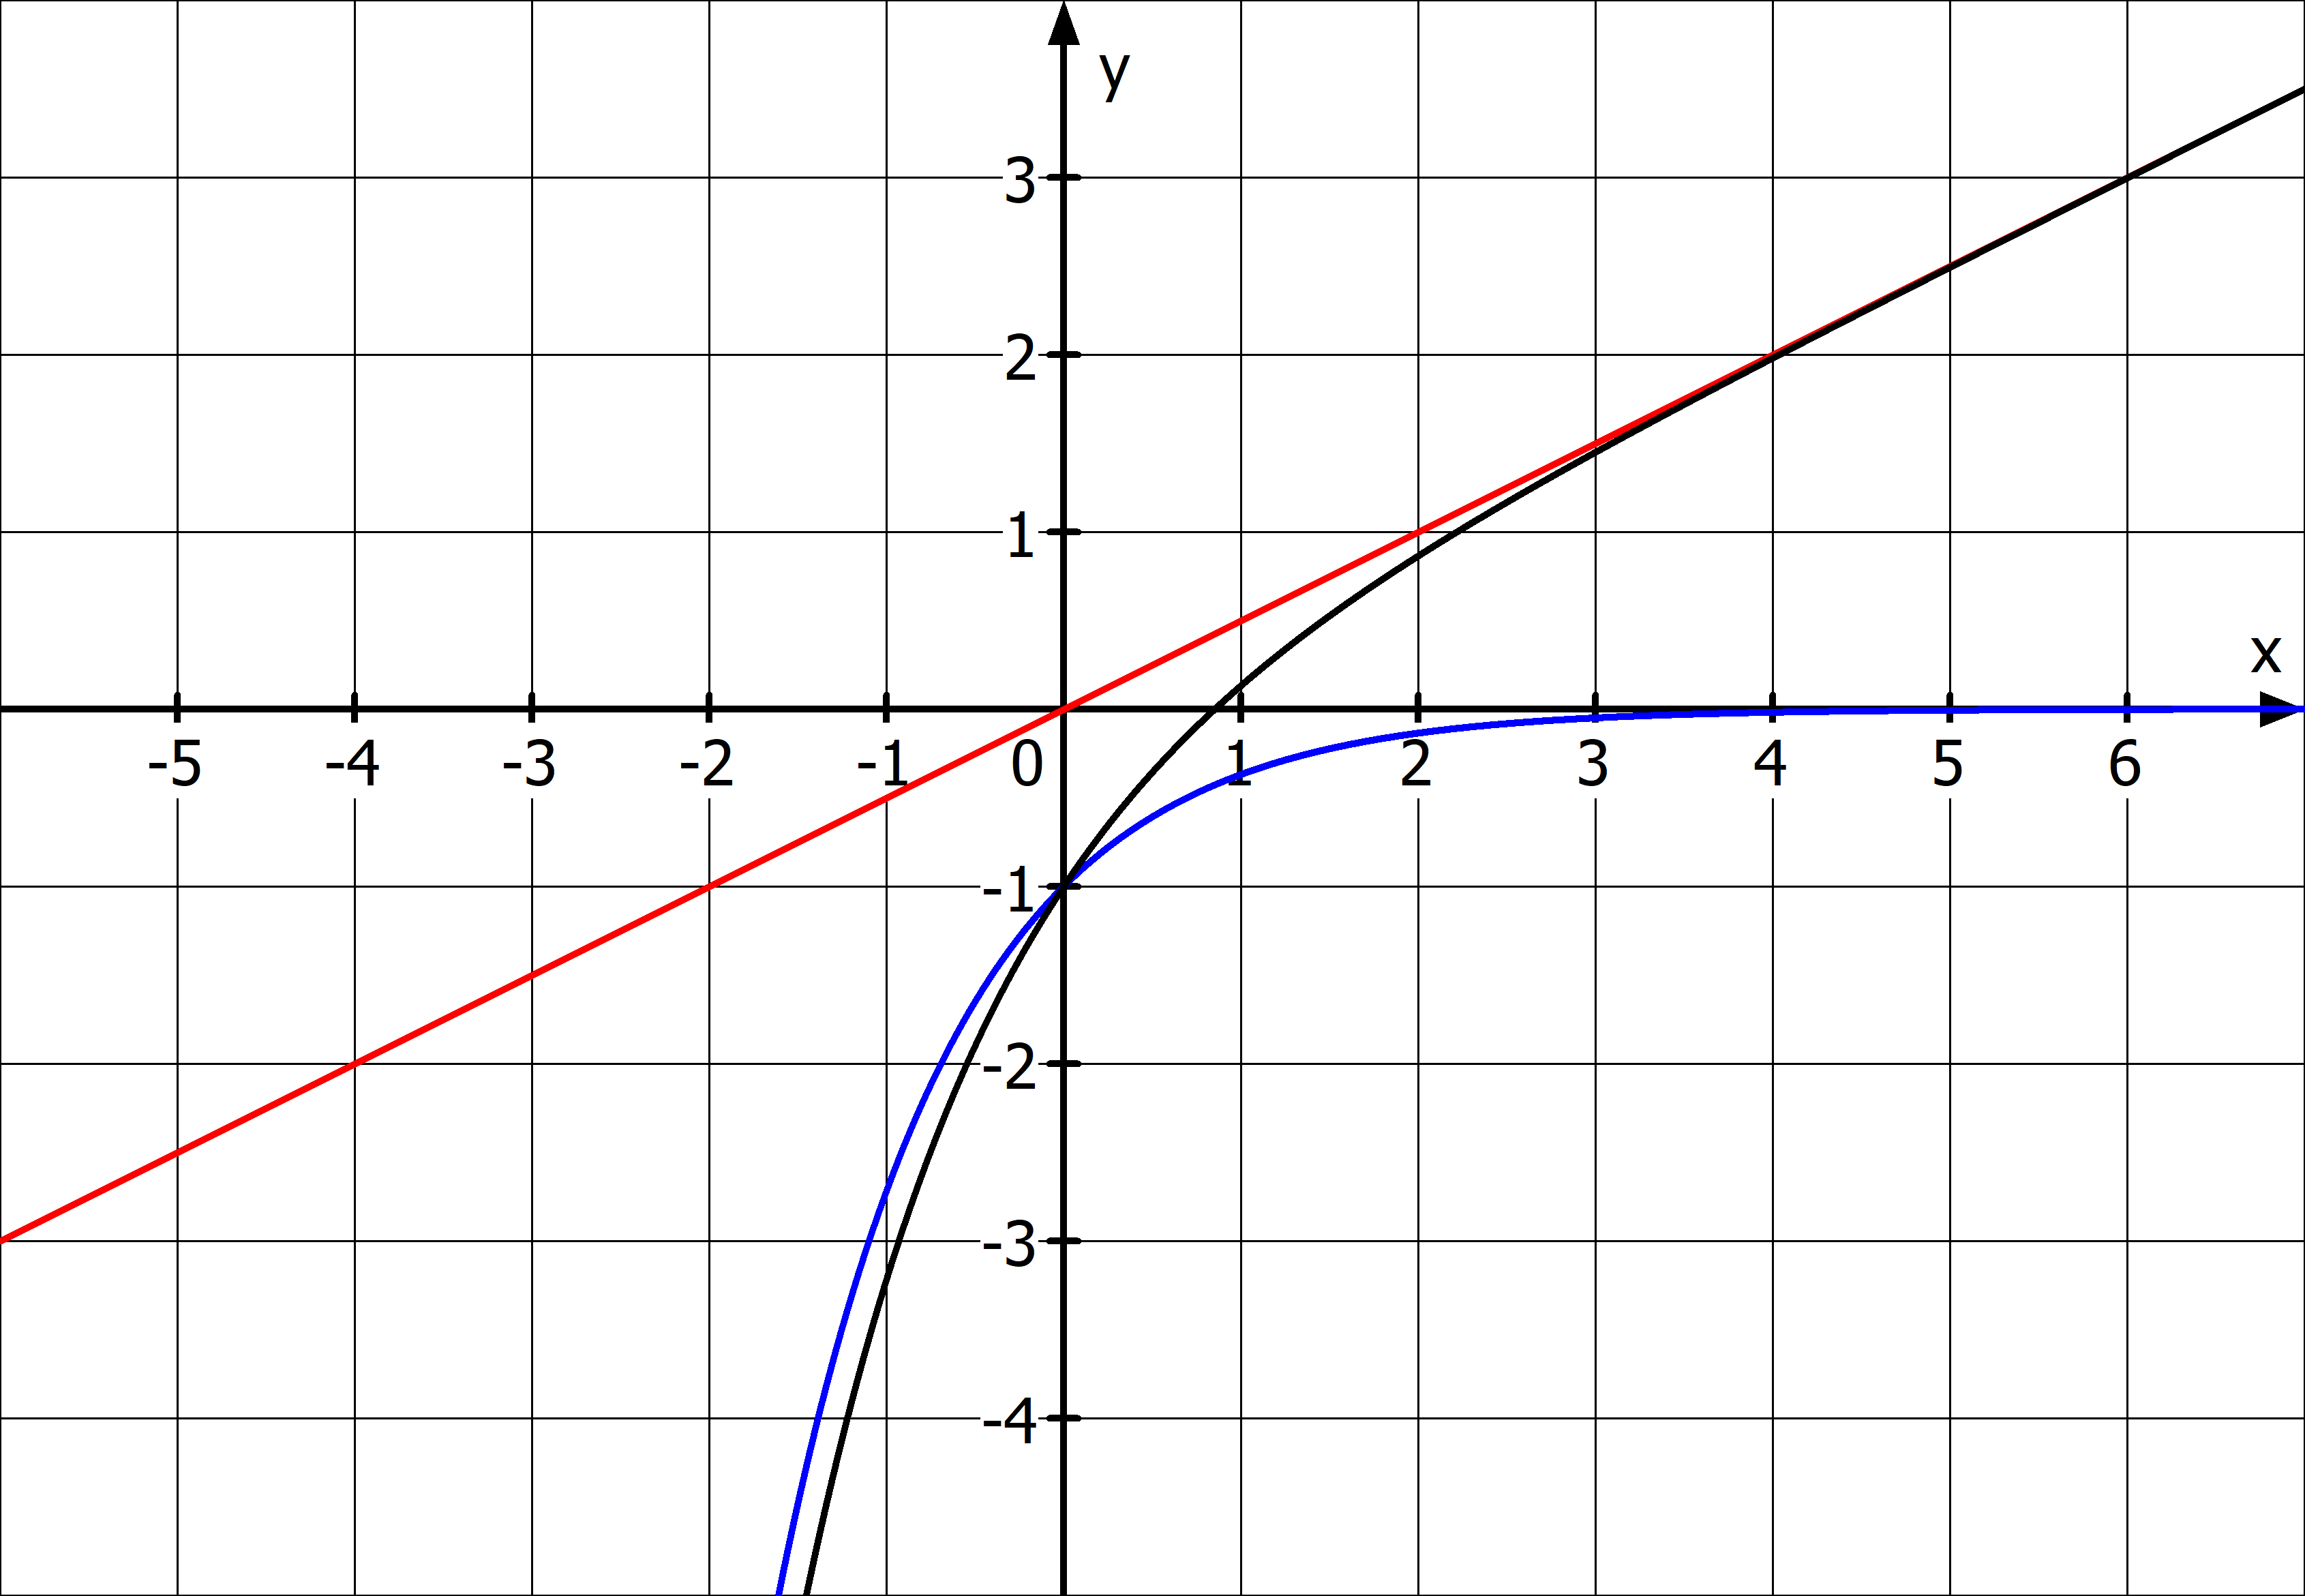
\includegraphics[width=\linewidth]{\eFkt/pics/schiefeAsymptoteA2.png}
				\end{minipage}
				\item \(f_3(x)=-e^{x}-\frac{2}{3}x+1\)

                \begin{minipage}[t]{0.87\textwidth}
					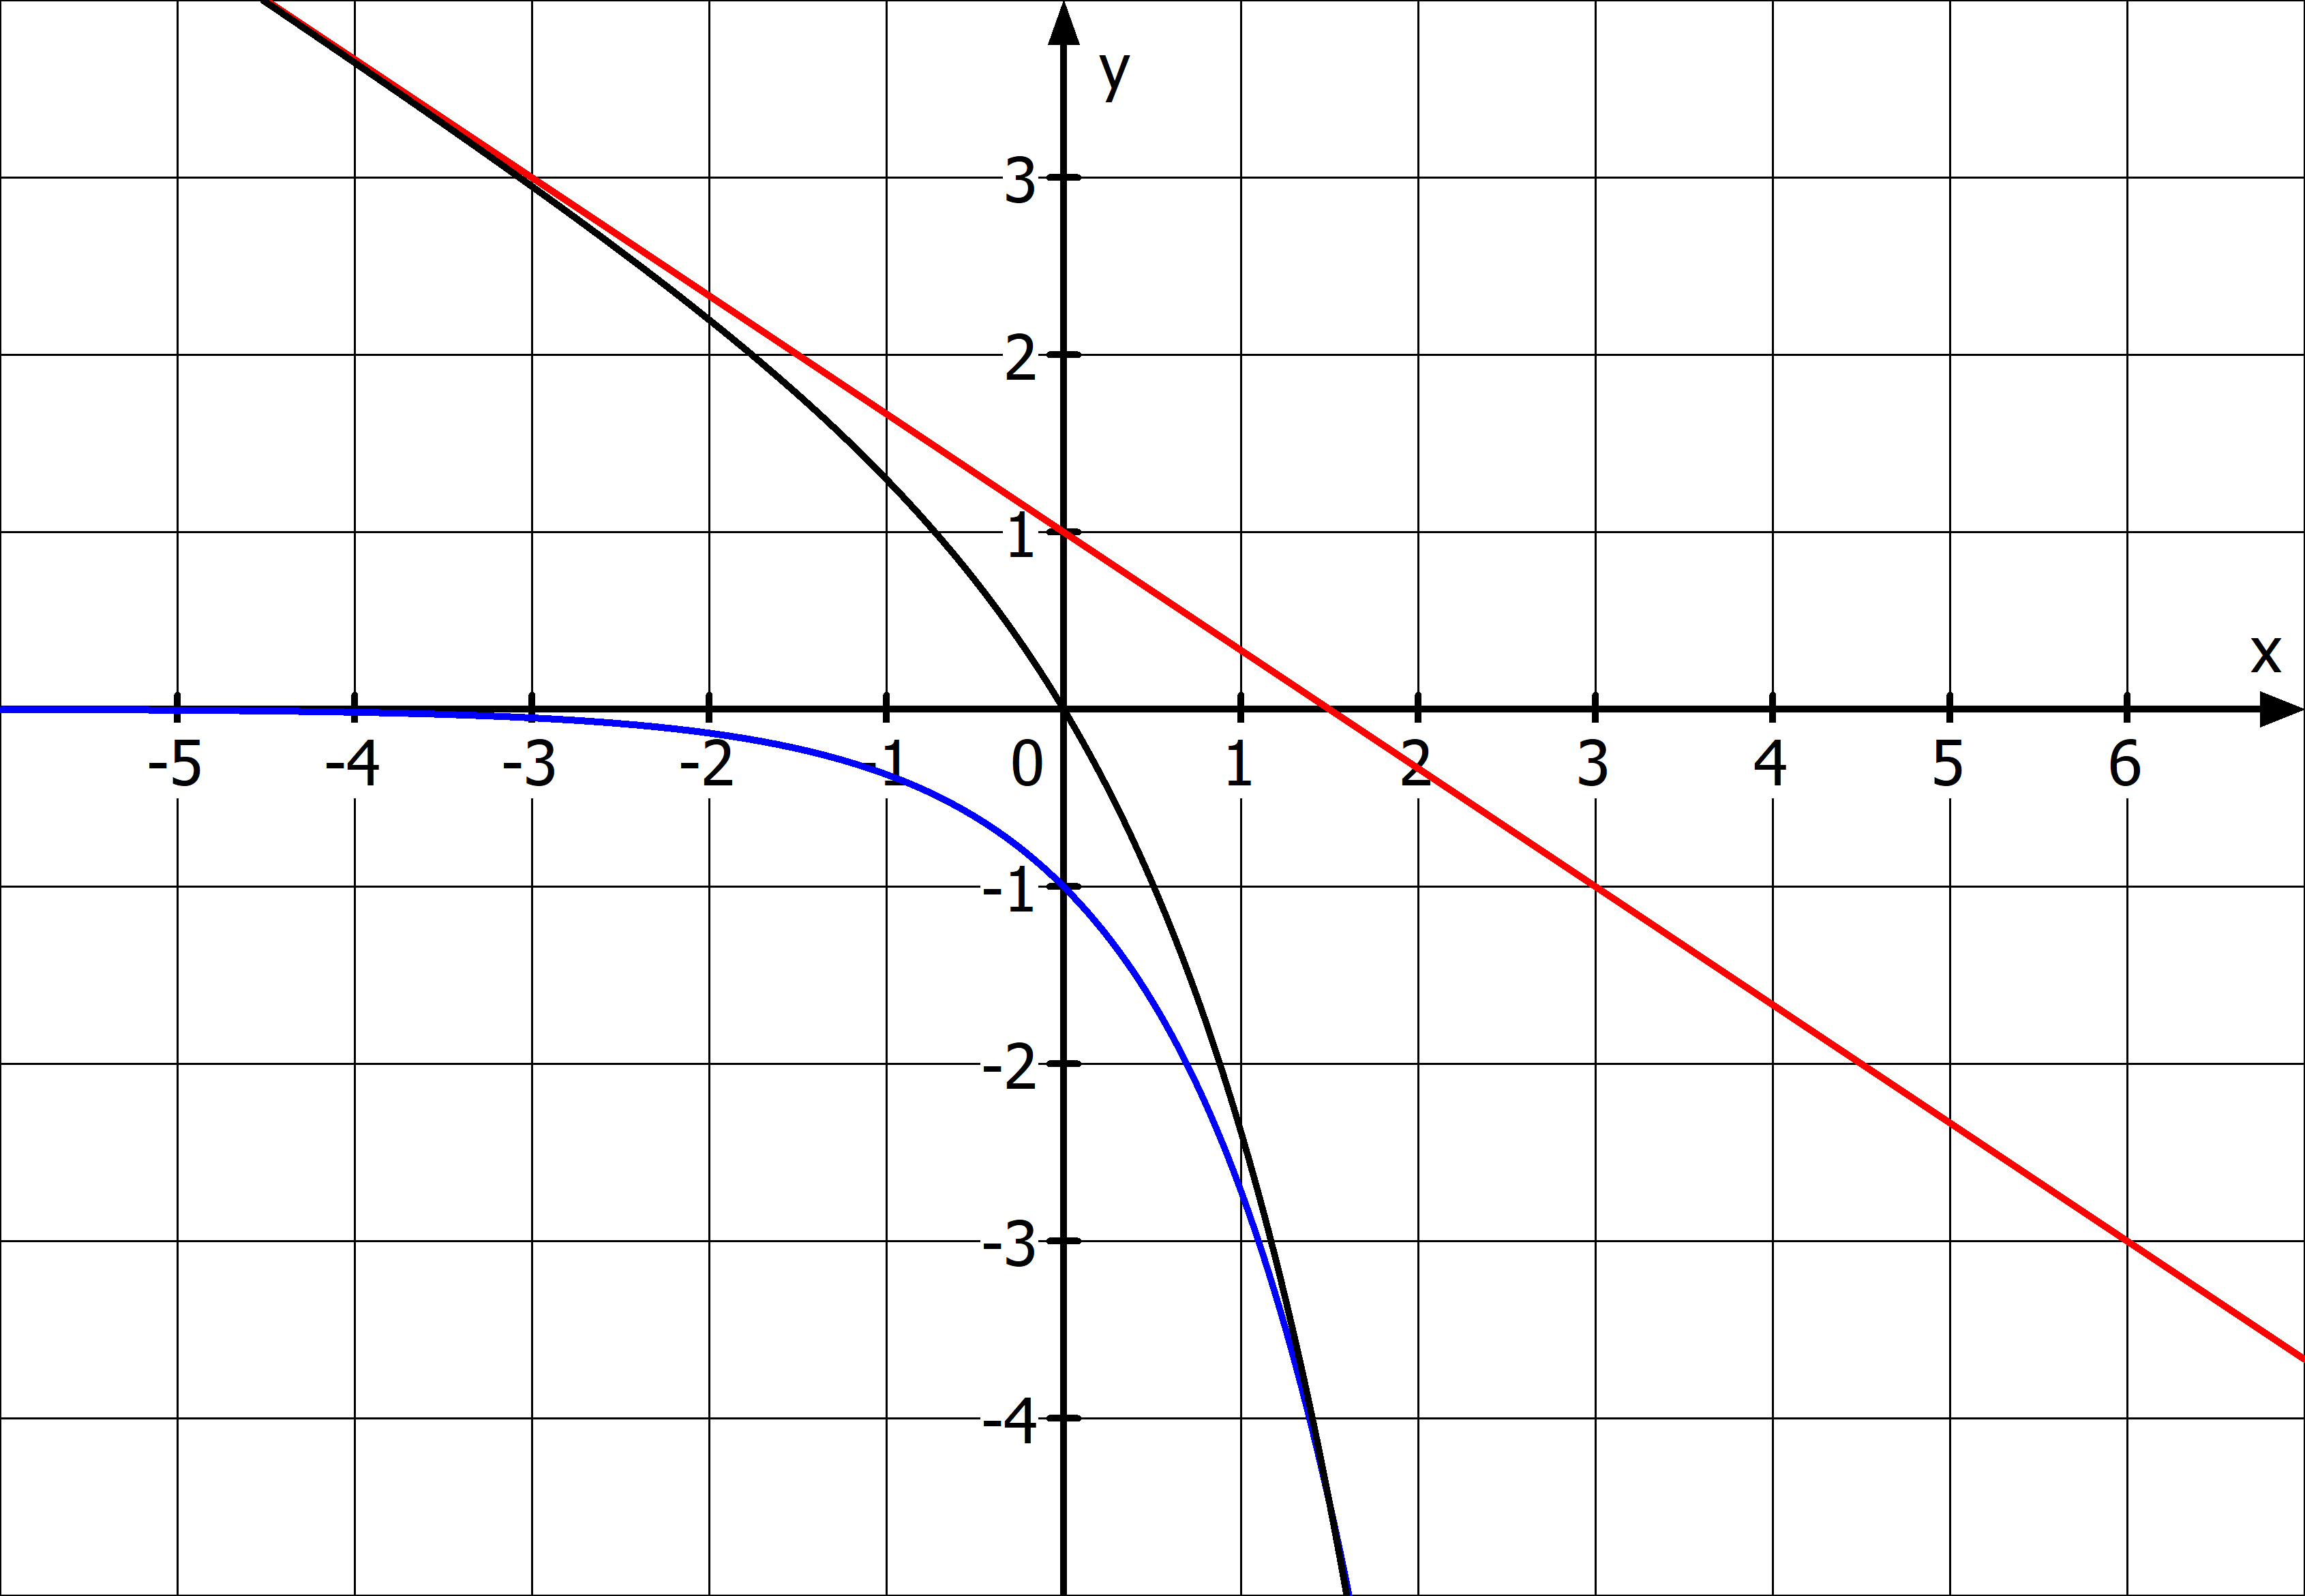
\includegraphics[width=\linewidth]{\eFkt/pics/schiefeAsymptoteA3.png}
				\end{minipage}
				\item \(f_4(x)=-2e^{-x}-2x+1\)

                \begin{minipage}[t]{0.87\textwidth}
					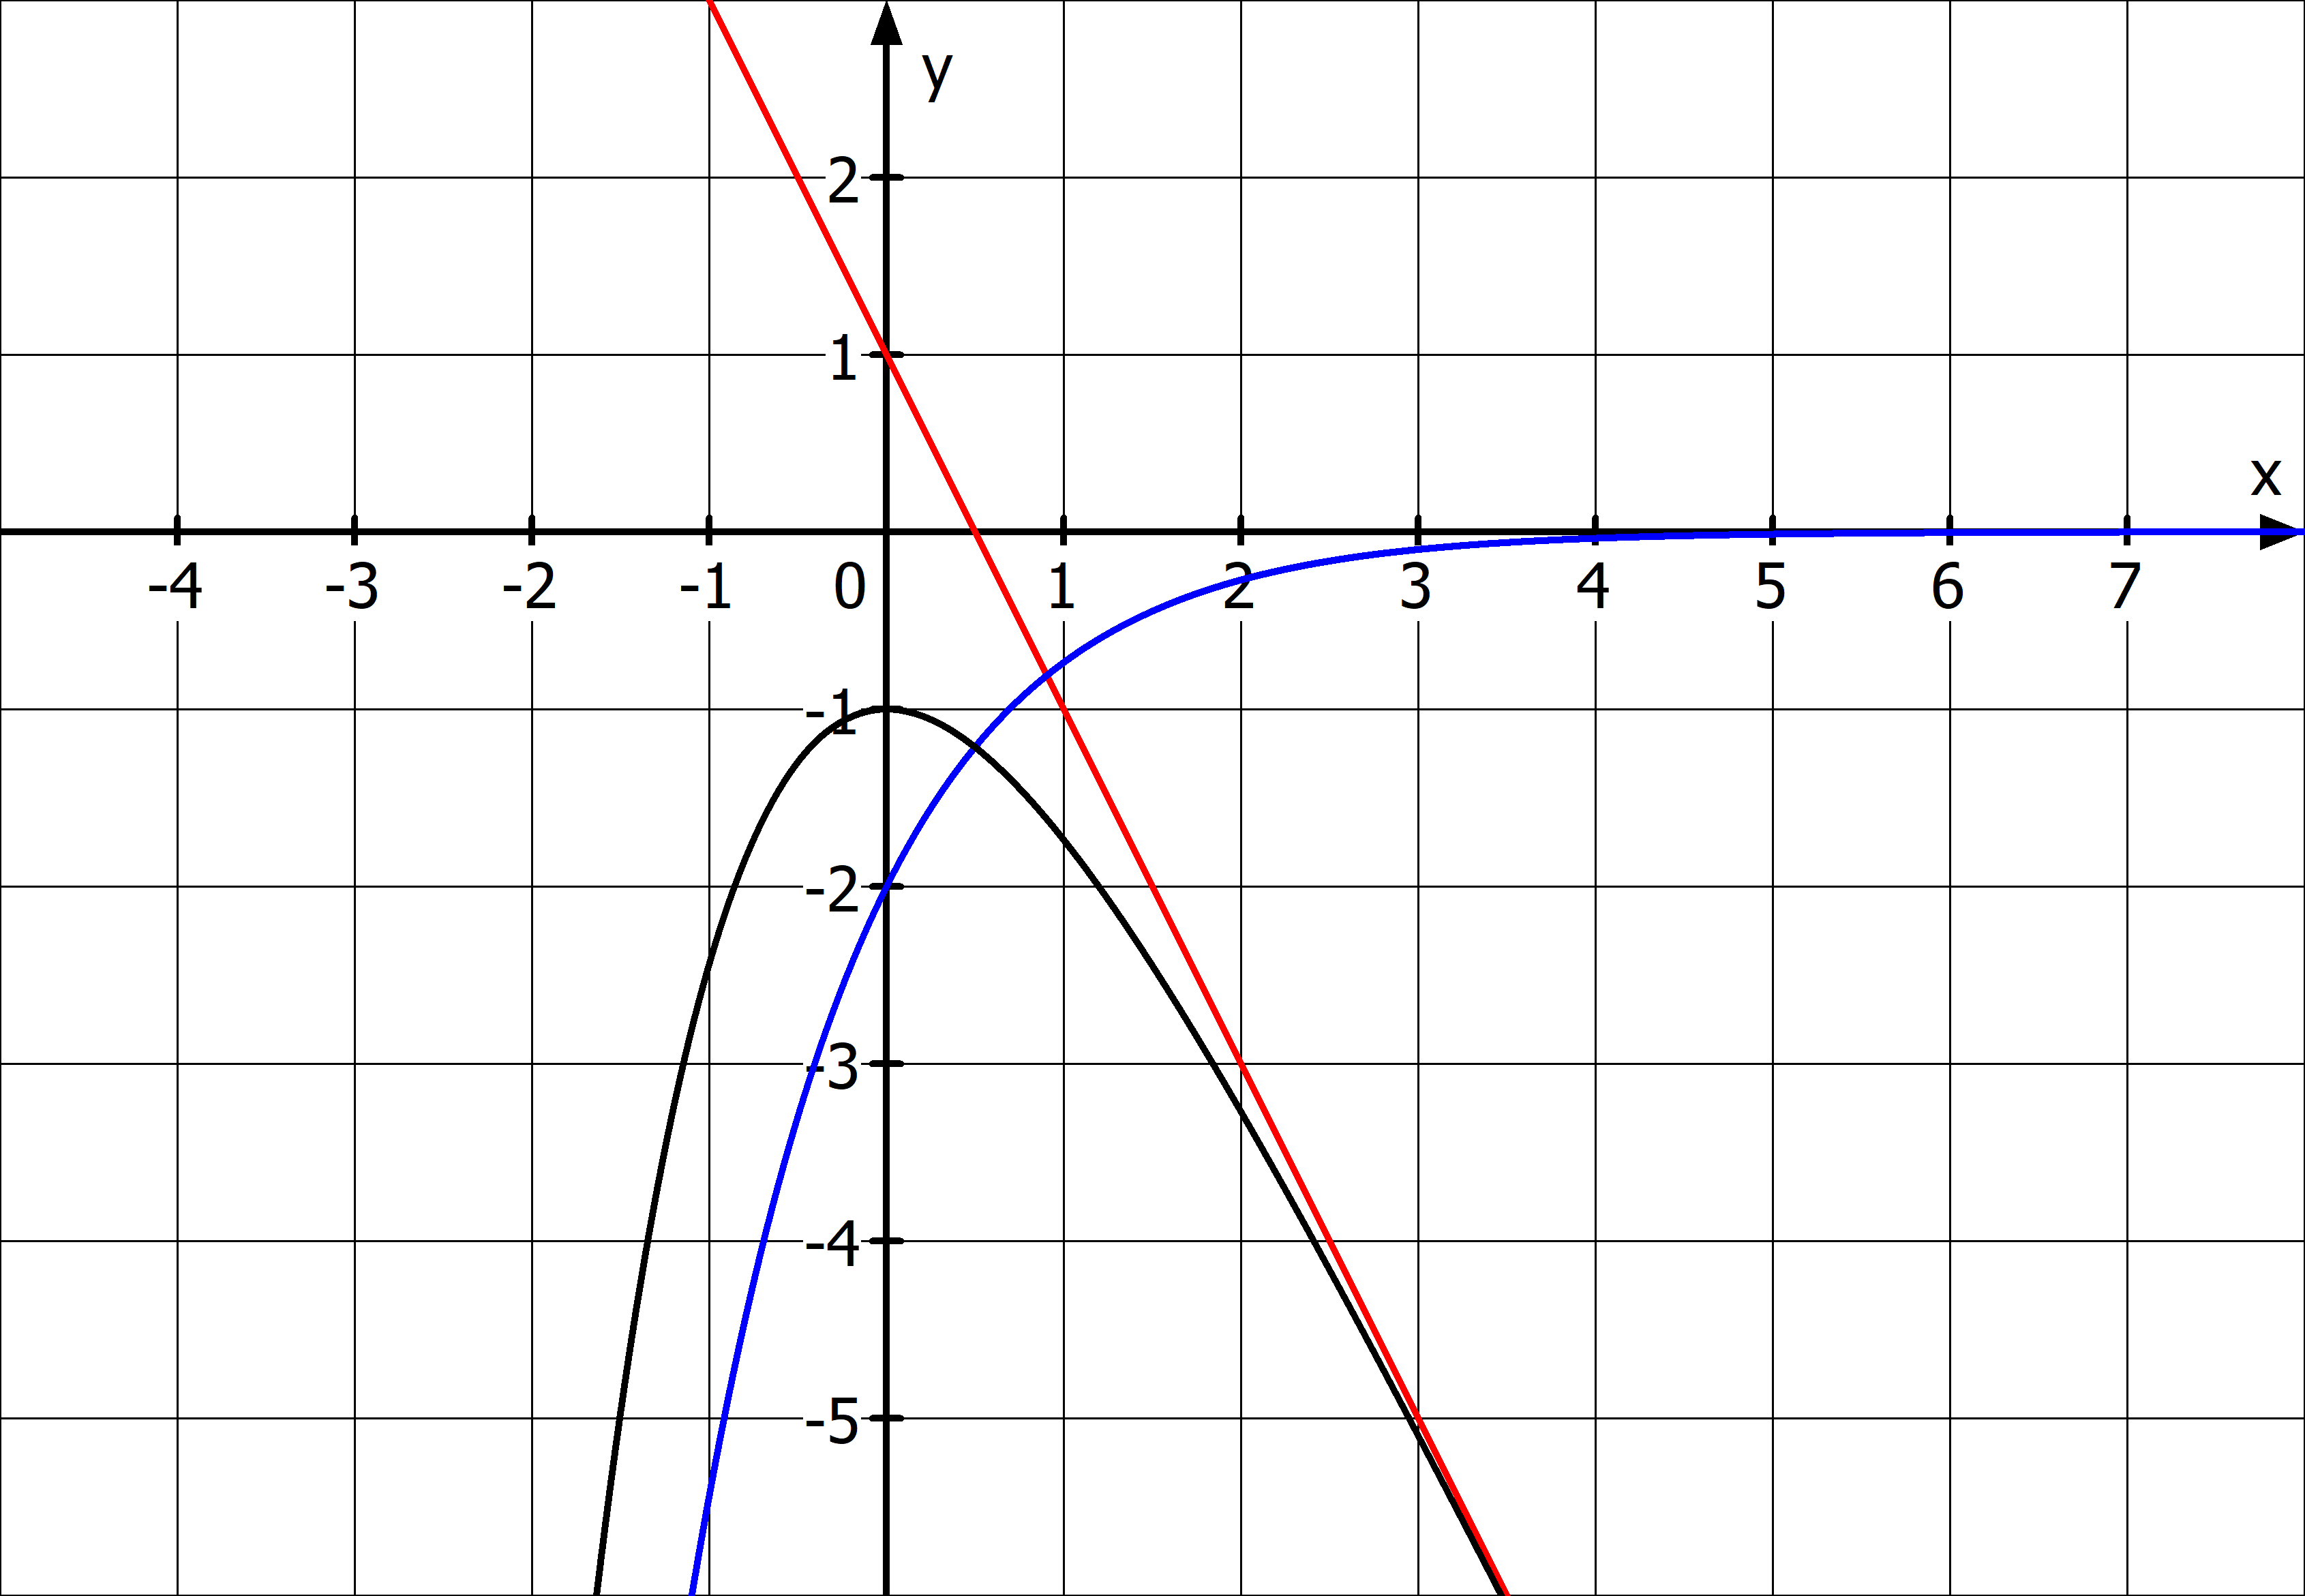
\includegraphics[width=\linewidth]{\eFkt/pics/schiefeAsymptoteA4.png}
				\end{minipage}
			\end{enumerate}
		\end{minipage}%
		\begin{minipage}{0.5\textwidth}
			\begin{enumerate}[label=\alph*)]
				\setcounter{enumi}{4}
				\item \(f_5(x)=3e^{1,4x}+\frac{3}{4}x-1\)

                \begin{minipage}[t]{0.87\textwidth}
					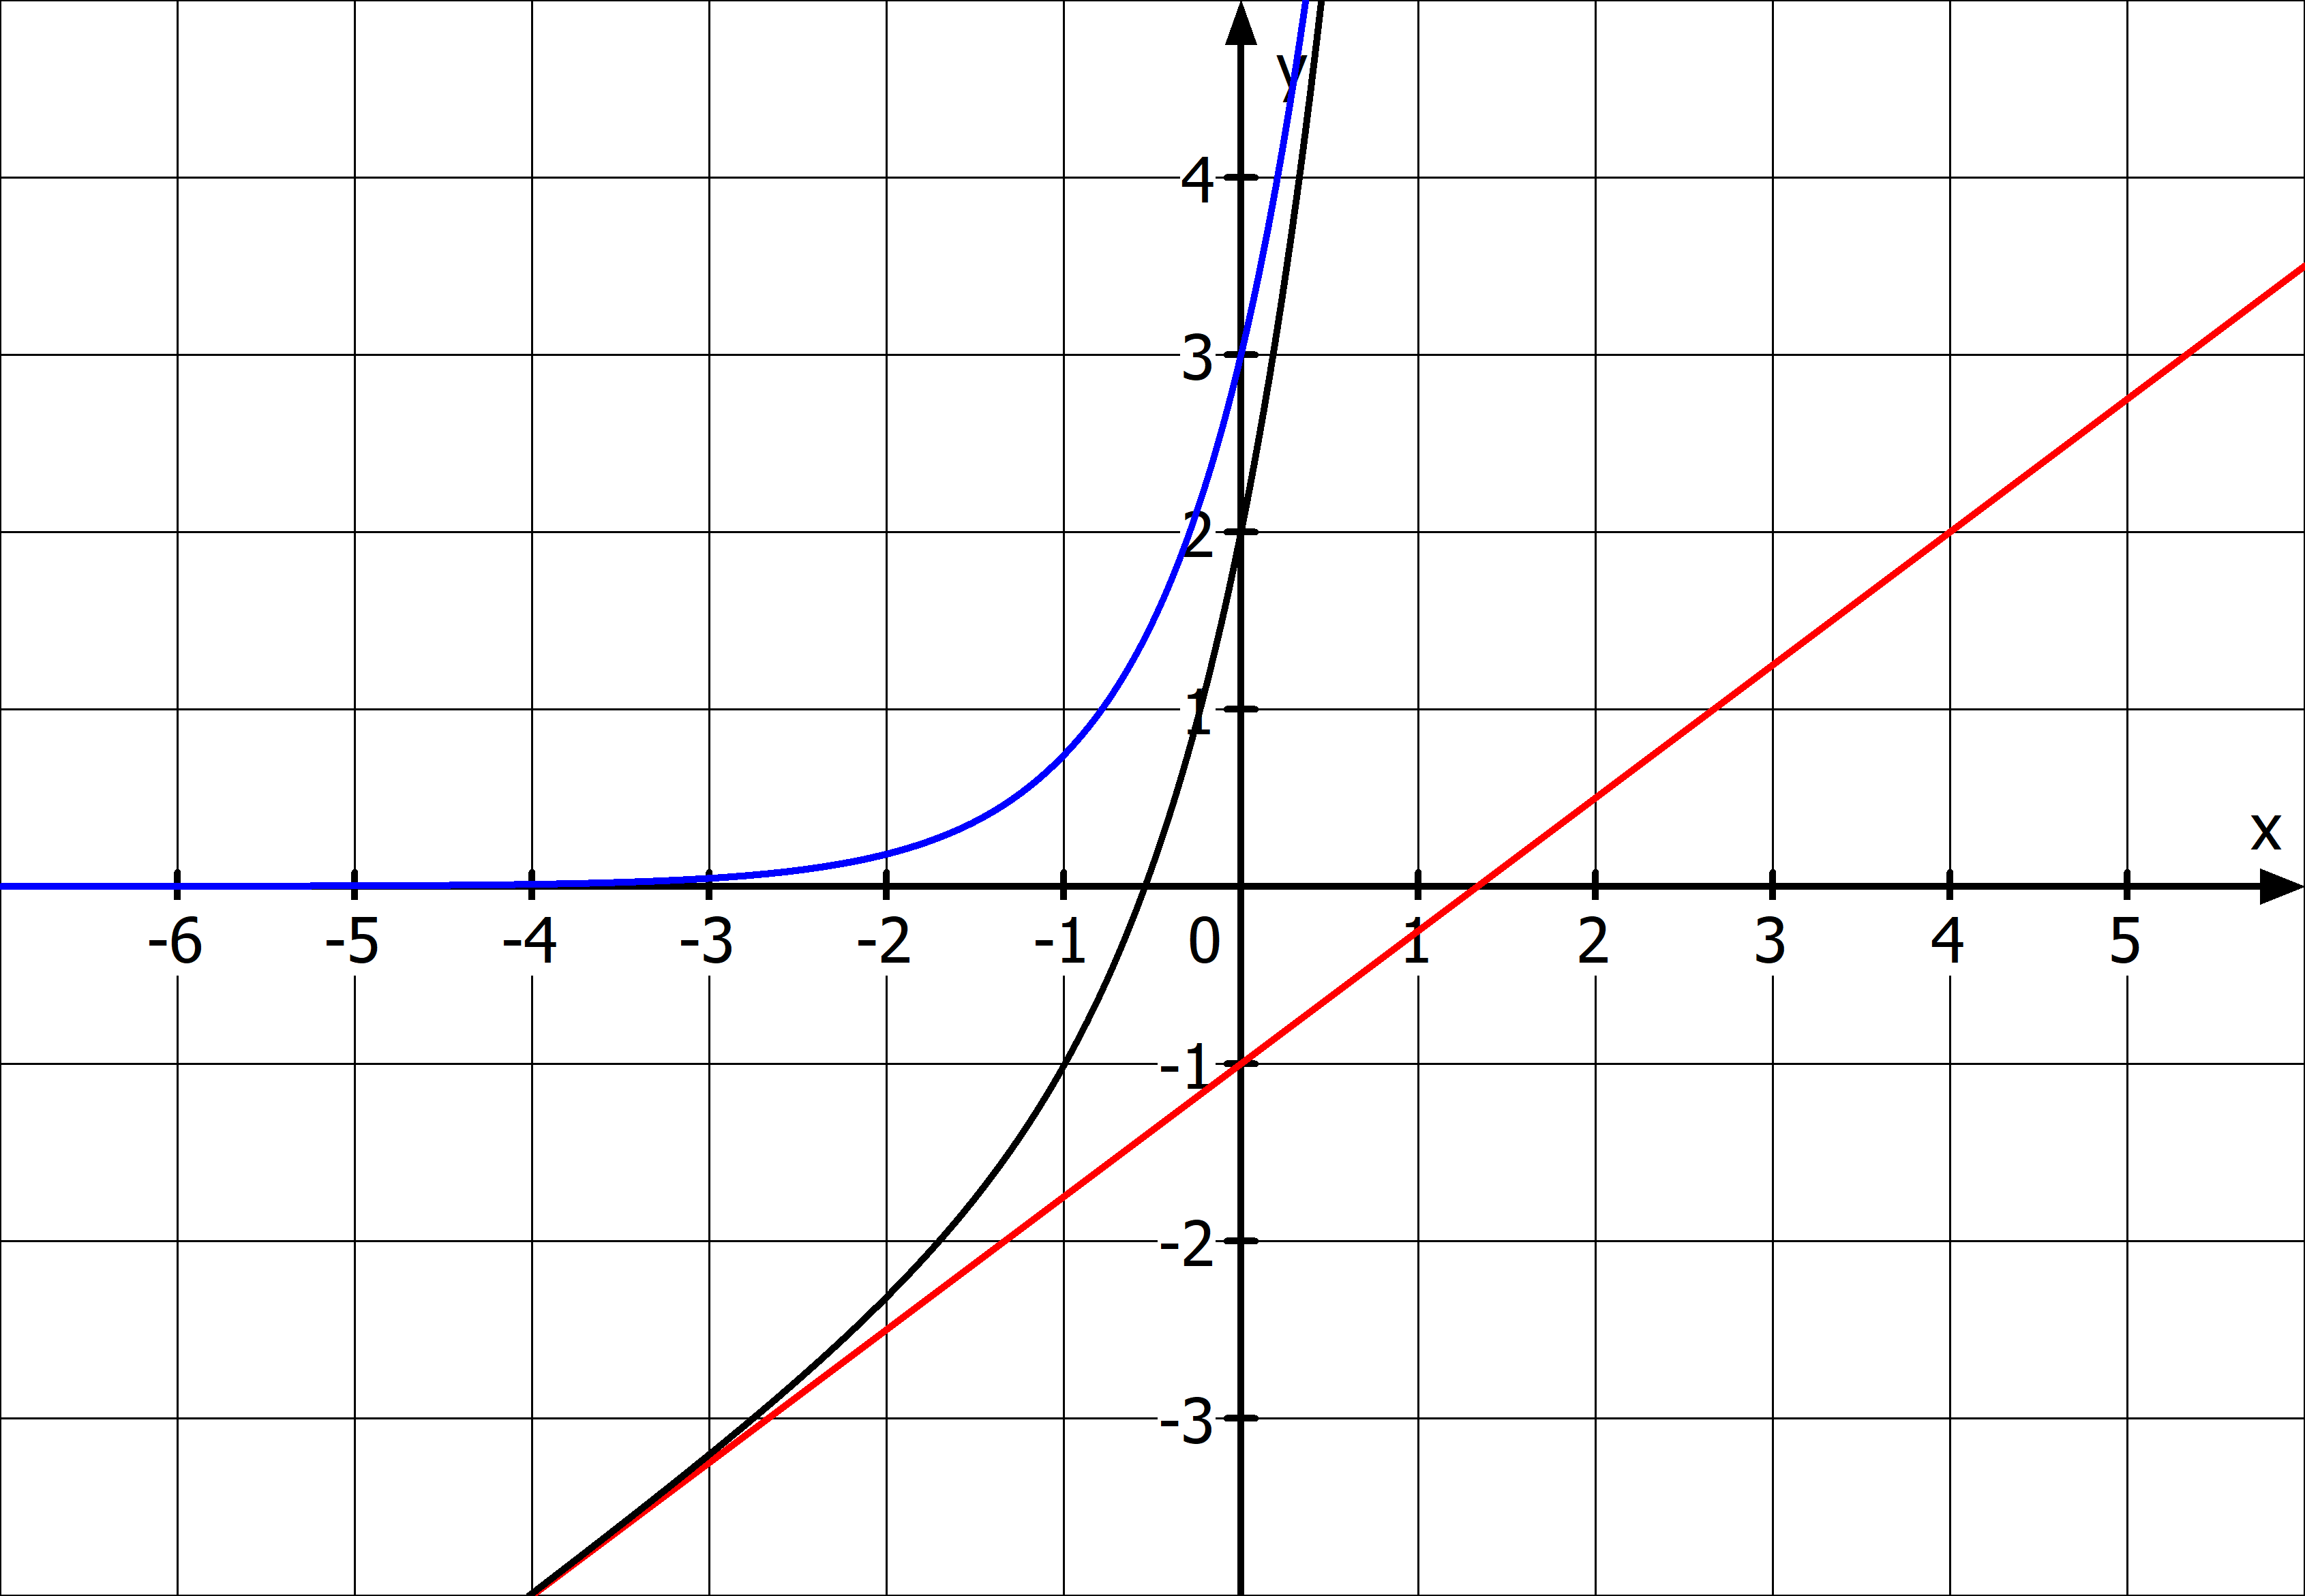
\includegraphics[width=\linewidth]{\eFkt/pics/schiefeAsymptoteA5.png}
				\end{minipage}
				\item \(f_6(x)=e^{2x}+0,4x-3\)

                \begin{minipage}[t]{0.87\textwidth}
					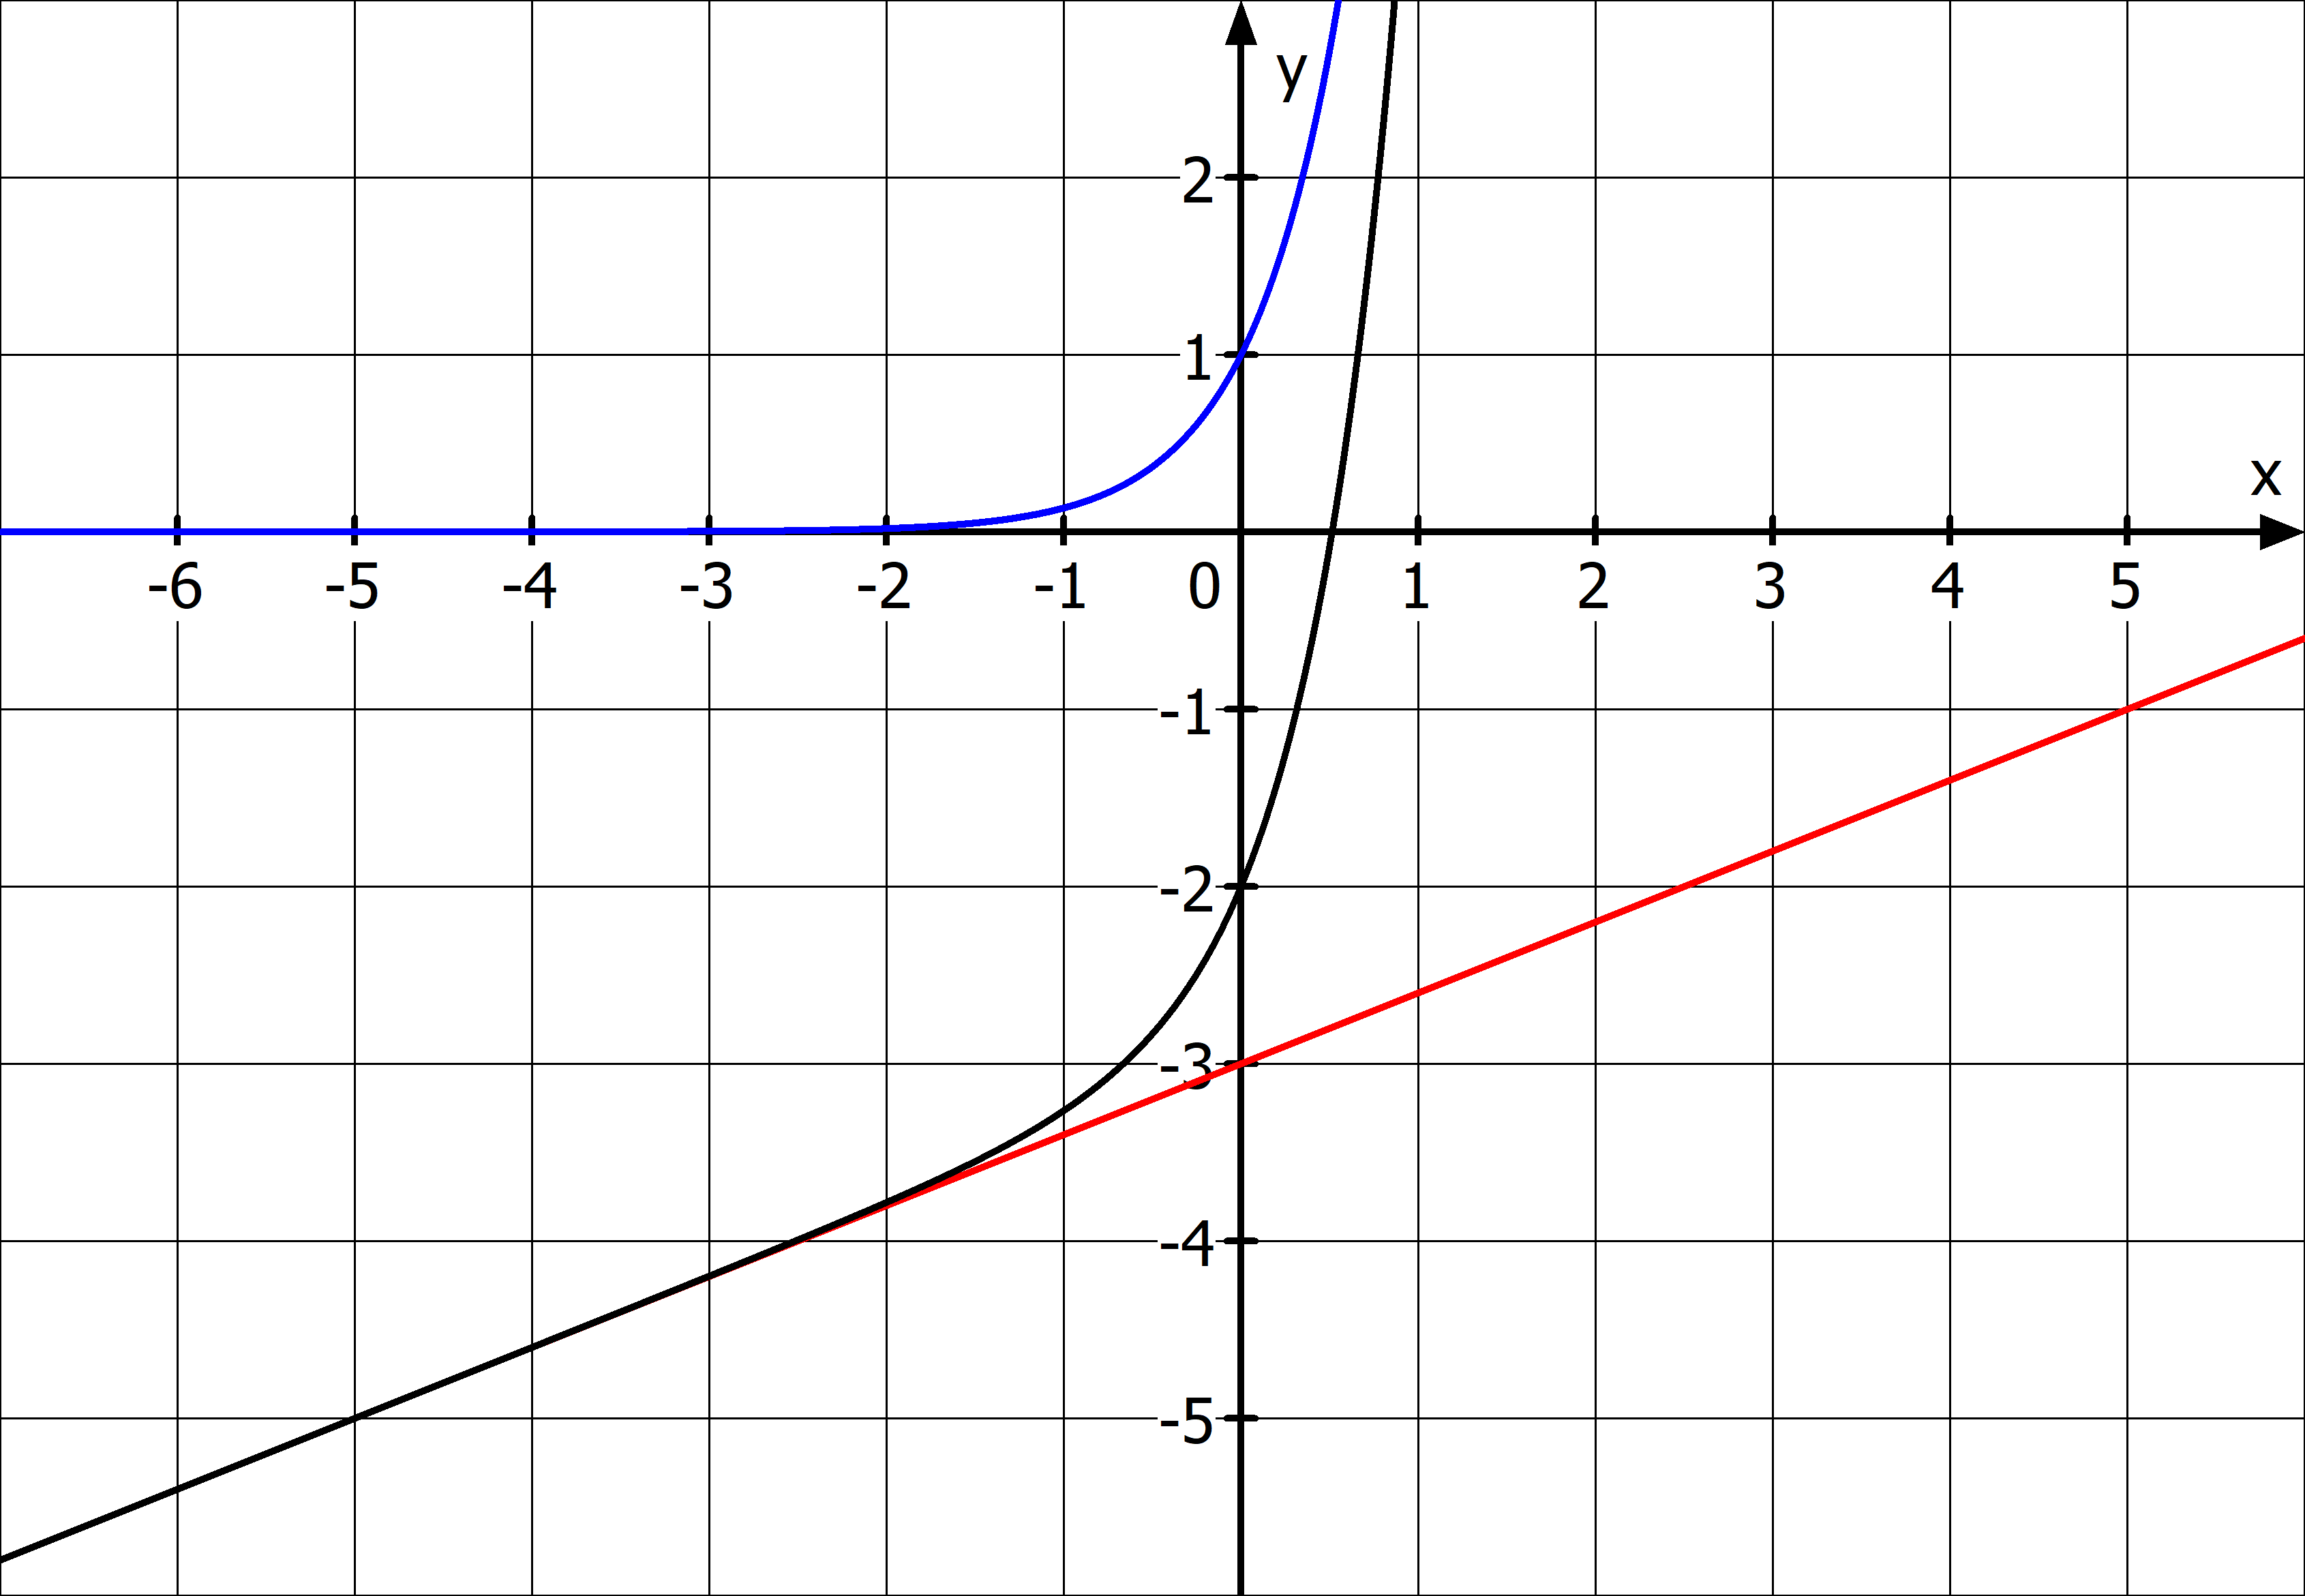
\includegraphics[width=\linewidth]{\eFkt/pics/schiefeAsymptoteA6.png}
				\end{minipage}
				\item \(f_7(x)=-3e^{-0,5x}-x\)

                \begin{minipage}[t]{0.87\textwidth}
					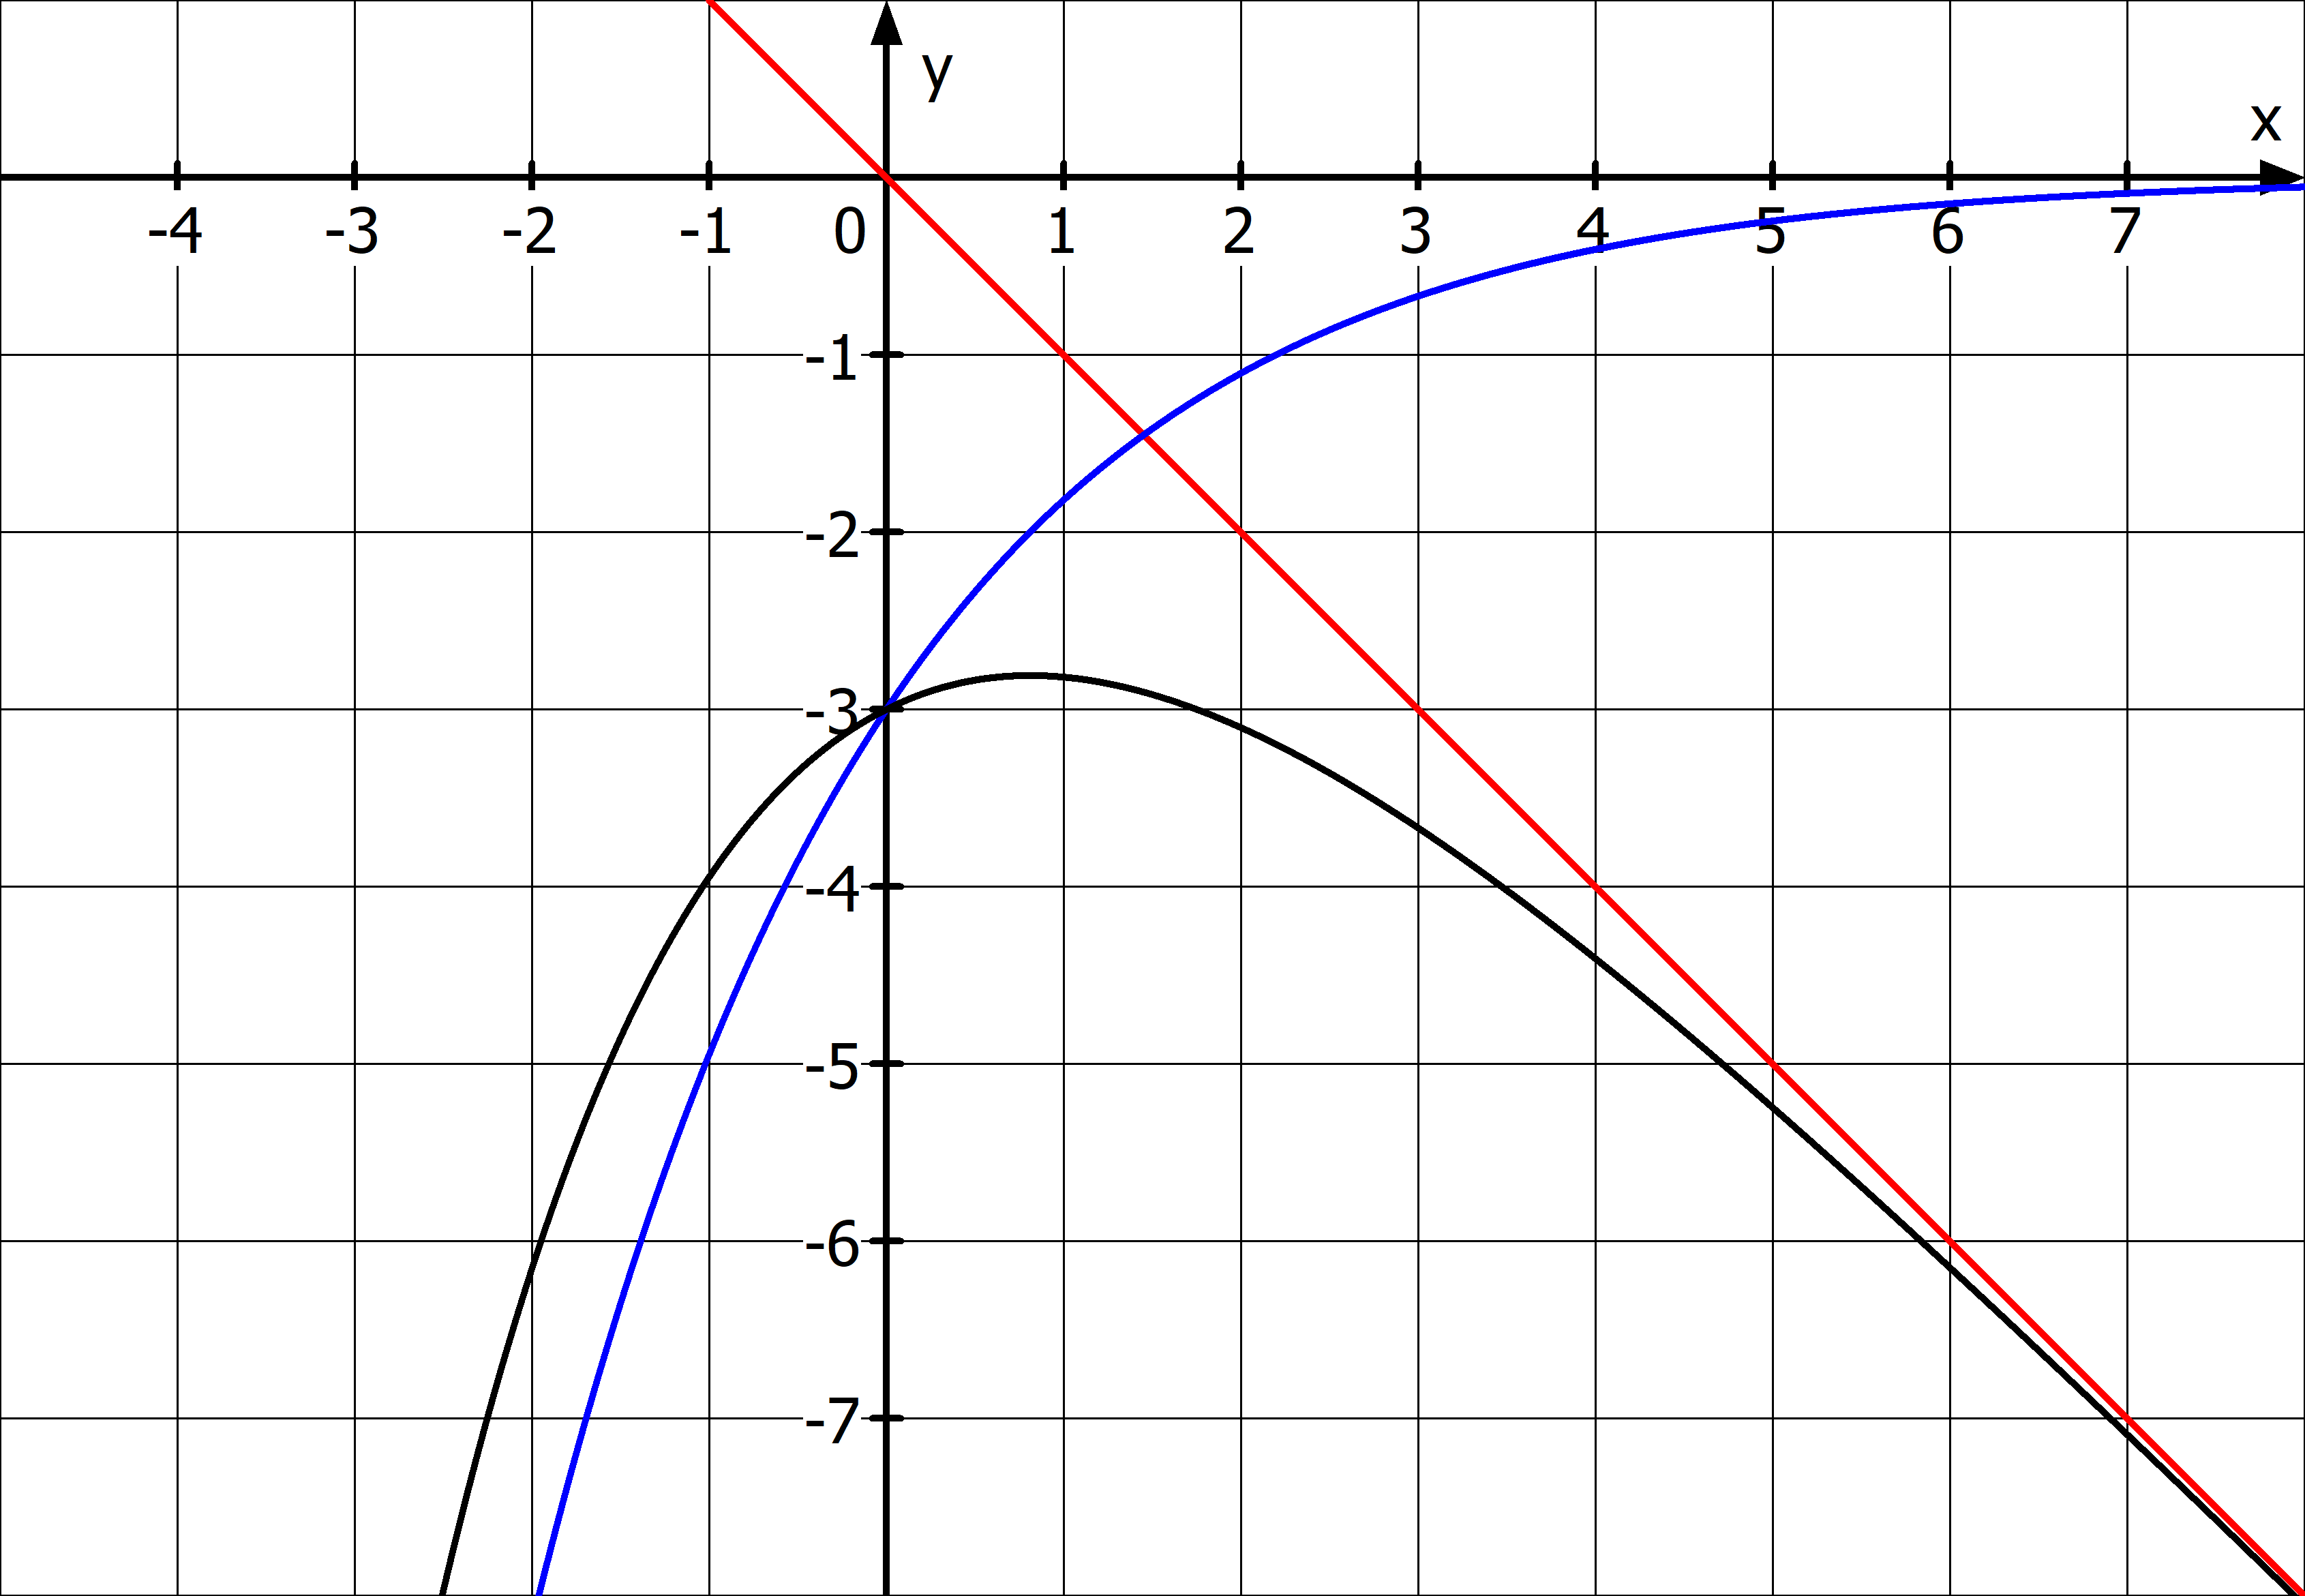
\includegraphics[width=\linewidth]{\eFkt/pics/schiefeAsymptoteA7.png}
				\end{minipage}
				\item \(f_8(x)=-2e^{4x}+\frac{4}{3}x+5\)

                \begin{minipage}[t]{0.87\textwidth}
					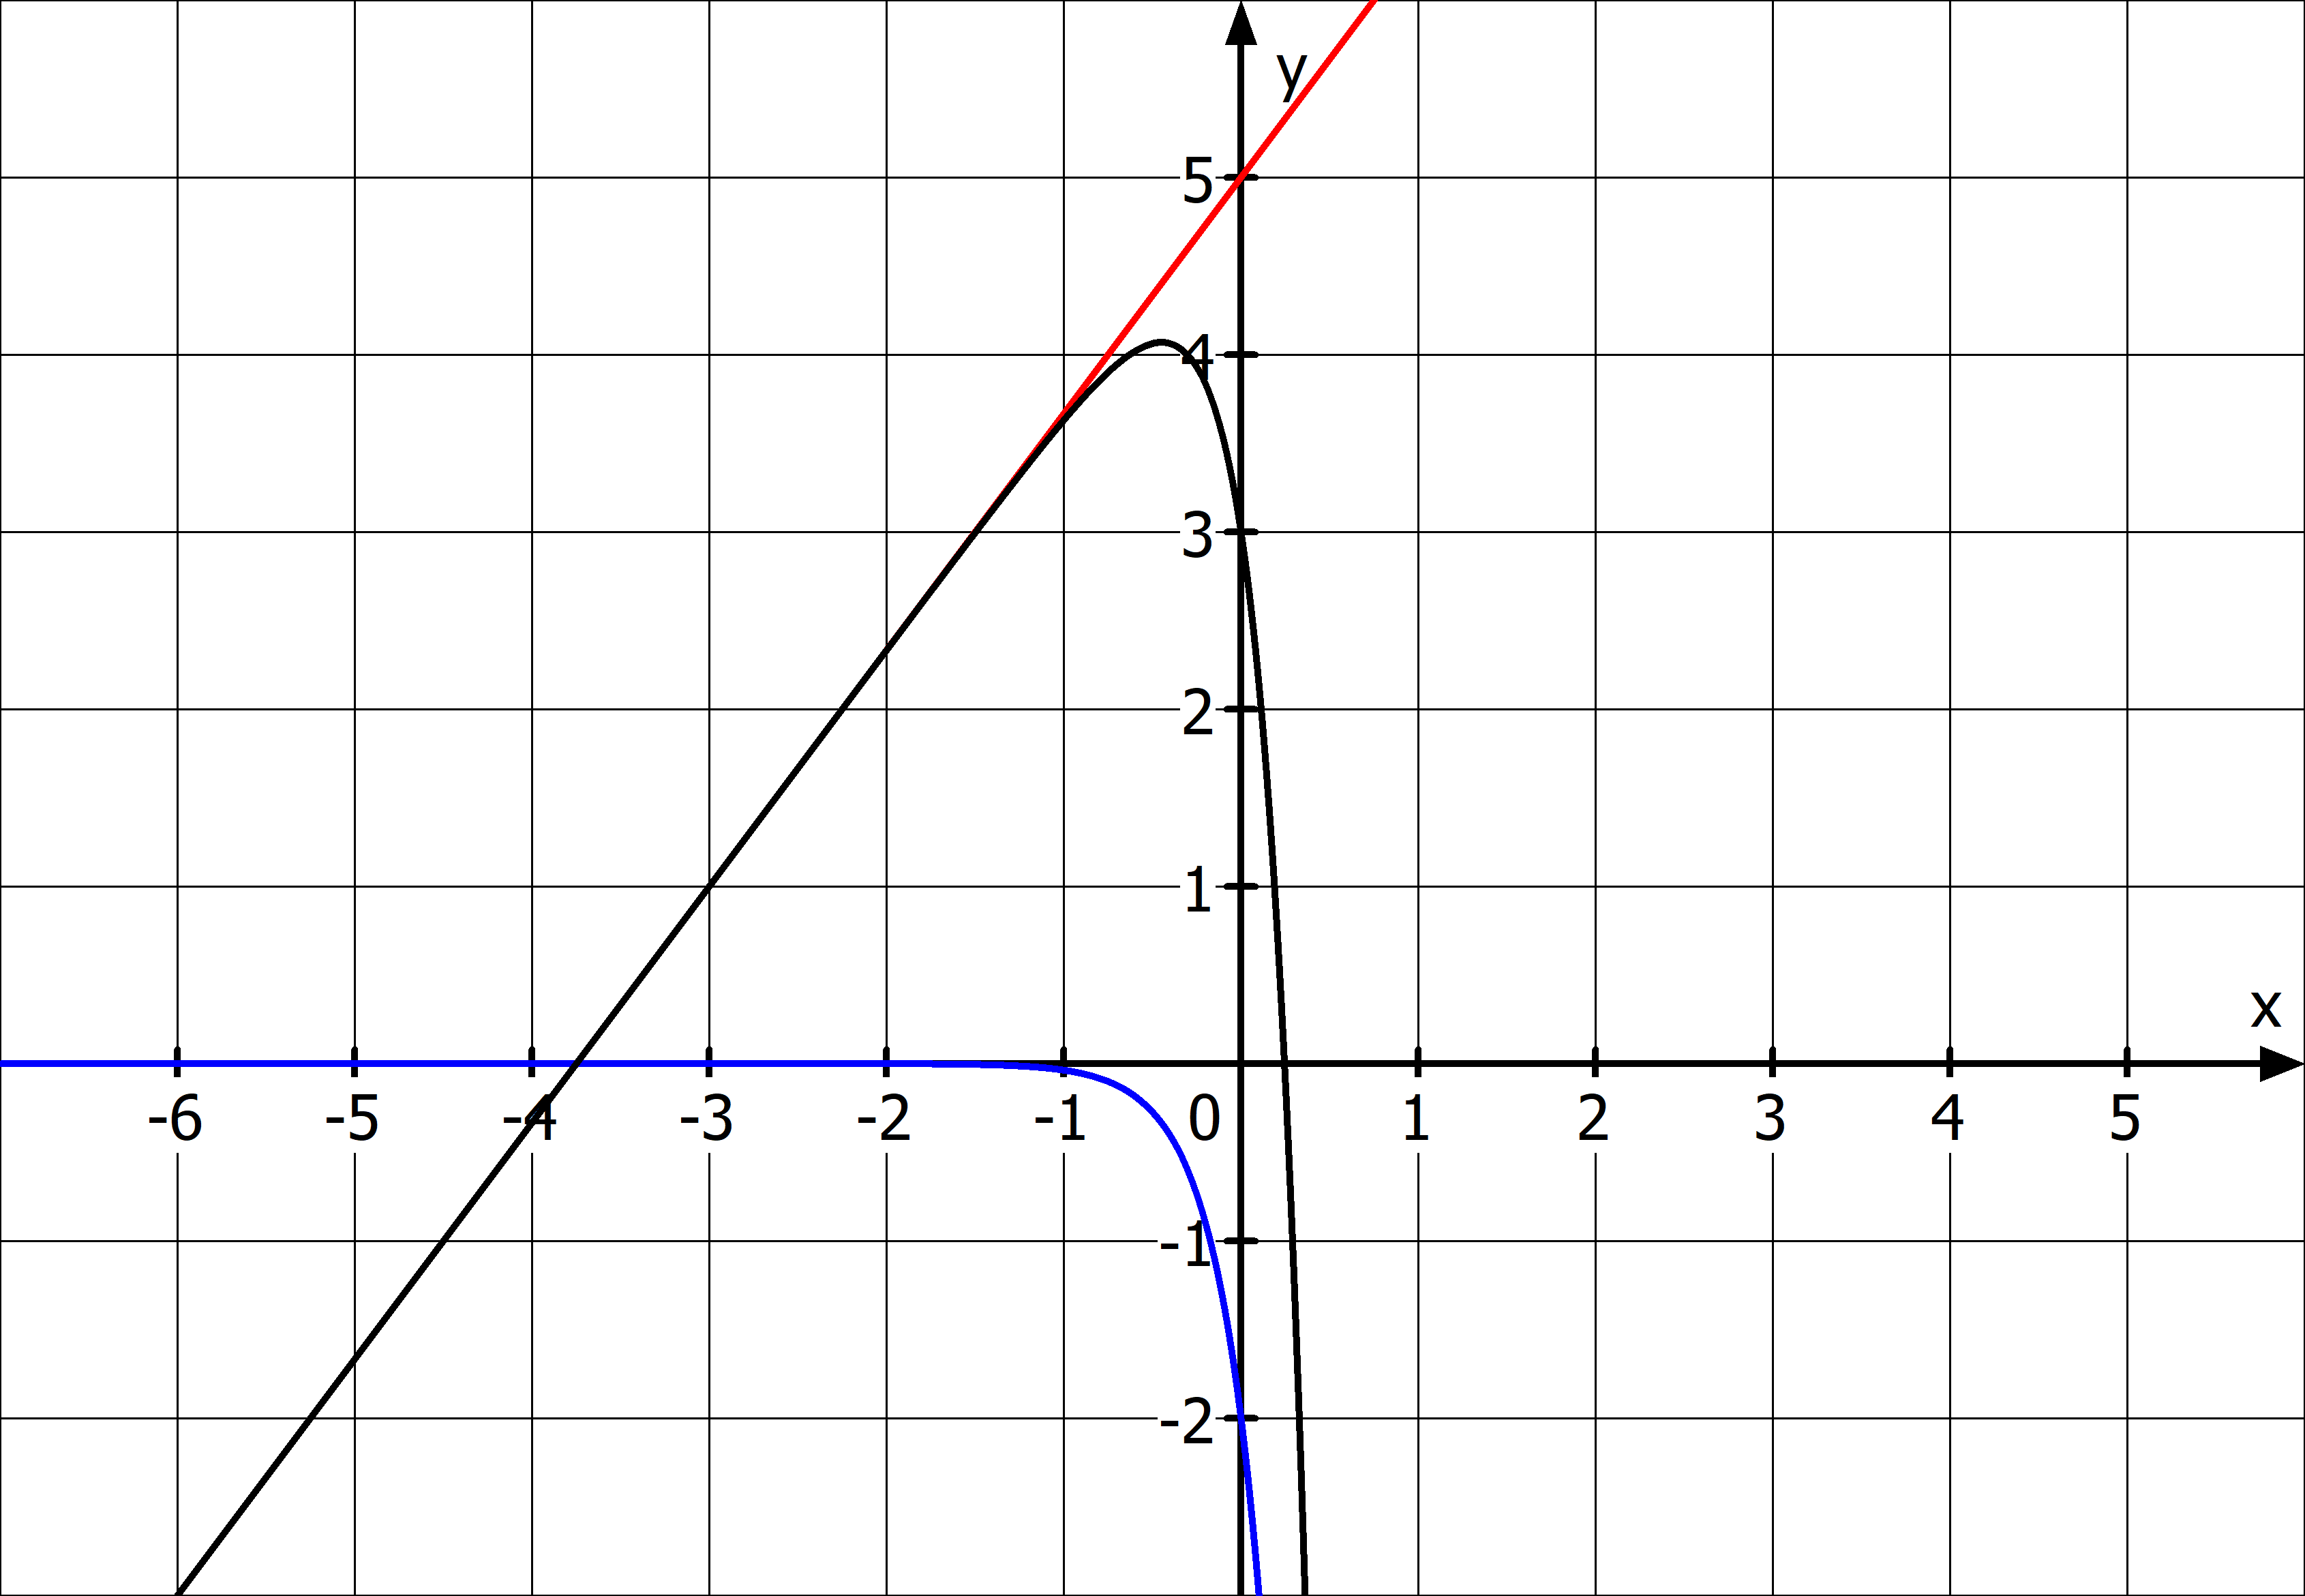
\includegraphics[width=\linewidth]{\eFkt/pics/schiefeAsymptoteA8.png}
				\end{minipage}
			\end{enumerate}
		\end{minipage}%
	\end{minipage}
\end{Answer}